\chapter{Modellierung und Zustandsraumdarstellung des Doppelpendels}

Die Grundlage f�r die Simulation des inversen Doppelpendels bilden die dynamischen Bewegungsgleichungen des Systems. In diesem Kapitel wird auf die Herleitung der Gleichungen eingegangen. In einem ersten Schritt werden die Bewegungsgleichungen mithilfe der Lagrange'schen Gleichungen 2. Art hergeleitet. Im Anschluss wird aus den Bewegungsgleichungen die Zustandsraumdarstellung abgeleitet. Diese ist f�r die hier angewendeten Regelungskonzepte des Doppelpendels notwendig.

\section{Dynamische Gleichungen}

Der generelle Aufbau des inversen Doppelpendels kann \bild{DPskizze} entnommen werden. Das mechatronische System besteht aus einem Wagen und zwei miteinander gekoppelte St�ben. Der Wagen wird auf einer Linearf�hrung bewegt und mit einem Motor angesteuert. Beide Pendelst�be sind rotatorisch miteinander gelagert, sodass sie Bewegungen nur in der x-y-Ebene durchf�hren k�nnen. F�r die Anwendung des Lagrange-Formalismus
\begin{equation}
	\label{eq:lagrange}
	\frac{	d}{dt} \frac{\partial L}{\partial \dot{q}_\mathrm{i}} - \frac{\partial L }{\partial q_\mathrm{i}} = Q_\mathrm{i}^\mathrm{n.k.}
\end{equation}

zur Bestimmung der Bewegungsgleichungen ist eine energetische Betrachtung des Systems n�tig. Hierbei repr�sentieren $ q_\mathrm{i} $ die generalisierten Koordinaten, $ \dot{q}_\mathrm{i} $ ihre zeitlichen Ableitungen und $ Q_\mathrm{i}^\mathrm{n.k.} $ eventuell auftretende nicht konservative Kr�fte. Die Lagrange-Funktion 
\begin{equation}
	\label{eq:lagrangeFunction}
	L = T- U
\end{equation}

setzt sich aus der kinetischen Energie $T$ des Systems und der potentiellen Energie $L$ zusammen. Die kinetische Energie 
\begin{equation}
	\label{eq:energyKin}
	T = \frac{1}{2} \sum_\mathrm{i = 0}^\mathrm{n} m_\mathrm{i} v_\mathrm{i}^{2} 
	+ \frac{1}{2} \sum_\mathrm{i = 1}^\mathrm{2} J_\mathrm{i}^\mathrm{S} \varphi_\mathrm{i}^2  
\end{equation}

besteht aus der translatorischen Bewegungsenergie der $ n $ Schwerpunkte und der Rotationsenergie der Pendelst�be. Die Tr�gheiten der Pendel werden �ber das Massentr�gheitsmoment eines d�nnen Stabes mit 

\begin{align*}
	J_\mathrm{i}^\mathrm{S} = \frac{1}{12} m_\mathrm{i} l_\mathrm{i}^2
\end{align*}

approximiert. Die potentielle Energie des Systems l�sst sich im vorliegenden Fall auf das H�henpotential

\begin{equation}
	\label{eq:energyPot}
	U = g\sum_\mathrm{i  = 0}^\mathrm{n}  m_\mathrm{i}  y_\mathrm{i}  
\end{equation} 

beschr�nken. Das Nullniveau des Potentials wird auf die H�he $ y_0 $ des Wagens gelegt, sodass sich die potentielle Energie wie folgt ergibt:

\begin{equation}
\label{eq:energyPotTotal}
U = ... = g \big( (\tfrac{1}{2} m_1 + m_2 + m_3 ) l_1 \cos(\varphi_1) + \tfrac{1}{2} m_2 l_2 \cos(\varphi_2) \big) \text{.}
\end{equation}

Bei der Modellierung des Doppelpendels ist die Betrachtung von vier Schwerpunkten, die \bild{DPskizze} zu entnehmen sind, notwendig. Neben den Schwerpunkten des Wagens und der beiden Pendel, die �ber die Indizes 0, 1 und 2 verf�gen, ist noch das Verbindungsgelenk der St�be zu beachten. Das Gelenk wird als Punktmasse behandelt mit dem Index 3 versehen. Damit werden die Position der Massen zu

\begin{align*}
	x_0 &= x, &
	y_0 &= 0, \\
	x_1 &= x_0 - \tfrac{1}{2} l_1 \sin(\varphi_1), & 
	y_1 &= \tfrac{1}{2}l_1 \cos(\varphi_1), \\
	x_2 &= x_0 -l_1 \sin(\varphi_1) -\tfrac{1}{2}l_2\sin(\varphi_2), &
	y_2 &= l_1 \cos(\varphi_1) + \tfrac{1}{2}l_2\cos(\varphi_2), \\
	x_3 & =x_0-l_1\sin(\varphi_1),  &
	y_3 &= l_1\cos(\varphi_1) %\text{.} 
\end{align*}

bestimmt. Zur Ermittlung der Schwerpunktgeschwindigkeiten werden die zeitlichen Ableitungen

\begin{align*}
	\dot{x}_0 &= \dot{x}, &
	\dot{y}_0 &= 0, \\
	\dot{x}_1 &= \dot{x}_0 - \tfrac{1}{2} l_1 \cos(\varphi_1) \dot{\varphi}_1, &
	\dot{y}_1 &= -\tfrac{1}{2} l_1 \sin(\varphi_1) \dot{\varphi}_1, \\
	\dot{x}_2 &= \dot{x}_0 - l_1 \cos(\varphi_1) \dot{\varphi}_1 -\tfrac{1}{2}l_2\cos(\varphi_2) \dot{\varphi}_2, & \dot{y}_2 &= -l_1 \sin(\varphi_1) \dot{\varphi}_1 - \tfrac{1}{2} l_2 \sin(\varphi_2) \dot{\varphi}_2, \\ 
	\dot{x}_3 &= \dot{x}_0 - l_1\cos(\varphi_1) \dot{\varphi}_1, &
	\dot{y}_3 &= -l_1 \sin(\varphi_1) \dot{\varphi}_1 \\
\end{align*}

ben�tigt. Die Ermittlung der Gesamtgeschwindigkeit in der $ x $-$ y $-Ebene unter Ber�cksichtigung von $ \dot{x}_0 = \dot{x} $ ist �ber eine Betragsbildung m�glich und liefert

\begin{align*}
	v_0^2 &= \dot{x}_0^2 + \dot{y}_0^2 = \dot{x}^2, \\
	v_1^2 &= \dot{x}_1^2 + \dot{y}_1^2 = \dot{x}^2 -l_1\cos(\varphi_1) \dot{x}_1 \dot{\varphi}_1 
	+ \tfrac{1}{4} l_1^2 \dot{\varphi}_1^2, \\
	v_2^2 &= \dot{x}_2^2 + \dot{y}_2^2 \\
	&= \dot{x}^2 + l_1 \dot{\varphi}_1^2 + \tfrac{1}{4} l_2^2 \dot{\varphi}_2^2
	- 2 \dot{x}^2 l_1 \cos(\varphi_1) \dot{\varphi}_1 - l_2 \dot{x} \cos(\varphi_2) \dot{\varphi_2}
	+ l_1 l_2 \cos(\varphi_1-\varphi_2) \dot{\varphi_1} \dot{\varphi_2}, \\
	v_3^2 &= \dot{x}_3^2 + \dot{y}_3^2 = \dot{x}^2 - 2 l_1 \cos(\varphi_1) \dot{x} \dot{\varphi_1} + l_1^2 \dot{\varphi_1} \text{.} 
\end{align*}

Somit ergibt sich die kinetische Energie des Systems mit der Gleichung~\ref{eq:energyKin} zu

\begin{align}
	\label{eq:energyKinTotal}
	\begin{split}
	T &= \frac{1}{2} (m_0 v_0^2 + m_1 v_1^2 + J_1^\mathrm{S} \varphi_1^2 + m_2 v_2^2 + J_2^\mathrm{S} \varphi_2^2 + m_3 v_3^2)  \\
	&= ... = \frac{1}{2} \Big( (m_0 + m_1 + m_2 + m_3) \dot{x}^2 + (\tfrac{1}{4} m_1 + m_2 + m_3) l_1^2 \dot{\varphi_1}^2  \\
	 &-(m_1 + 2m_2 + 2m_3 ) l_1 \dot{x} \cos(\varphi_1) \dot{\varphi_1} 
	+ m_2 (\tfrac{1}{4} l_2^2 \dot{\varphi_2}^2 - l_2 \dot{x} \cos(\varphi_2) \dot{\varphi_2} )  \\
	&+ l_1 l_2 \cos(\varphi_1-\varphi_2)\dot{\varphi_1}\dot{\varphi_2} + J_1^\mathrm{S} \dot{\varphi_1}^2
	+ J_2^\mathrm{S} \dot{\varphi_2}^2	\Big) \text{.}
	\end{split}
\end{align}

Mithilfe der Gleichungen~\ref{eq:energyKinTotal} und~\ref{eq:energyPotTotal} werden die Lagrange-Gleichungen 2. Art aufgestellt. In dem vorliegenden Fall werden drei generalisierte Koordinaten $ x $, $ \varphi_1$ und $ \varphi_2 $ verwendet.

\begin{align}
	\frac{d}{dt} \frac{\partial L }{\partial \dot{x}} - \frac{\partial L }{\partial x} &= F_\mathrm{a} - F_\mathrm{r} 	\label{eq:lagrangeX}  \\
	\frac{d}{dt} \frac{\partial L }{\partial \dot{\varphi_1}} - \frac{\partial L }{\partial \varphi_1} &= d_\mathrm{2} (\dot{\varphi_2} - \dot{\varphi_1}) - d_\mathrm{1} \dot{\varphi_1} \label{eq:lagrangePhi1} \\	
	\frac{d}{dt} \frac{\partial L }{\partial \dot{\varphi_2}} - \frac{\partial L }{\partial \varphi_2} &= -d_\mathrm{2} (\dot{\varphi_2} - \dot{\varphi_1}) \text{.} \label{eq:lagrangePhi2}
\end{align}

In \cite{Behm2016} werden zwei M�glichkeiten Regelung und Steuerung des mechatronischen Systems aufgezeigt. Zum einen kann der Wagen momentengesteuert bewegt werden. Hierbei wird ein Wunschmoment $ M_\mathrm{soll} $ an den Motor �bertragen. Bei der Umsetzung des Moments hat die Reibung der Linearf�hrung jedoch einen gro�en Einfluss auf die letztendliche Bewegung des Wagens. Zum anderen ist es m�glich, eine Sollgeschwindigkkeit $ v_\mathrm{soll} $ vorzugeben. Dies hat den Vorteil, dass die Reibung des Systems vernachl�ssigt werden kann. Au�erdem wird in \cite{Behm2016} aufgezeigt, dass bei der Regelung des inversen Einfachpendels mit Drehzahlvorgabe bessere Regelungsgebnisse erzielt werden. Aus diesen Gr�nden wird im folgenden die Wagenbeschleunigung $ \ddot{x} $ als Eingangsgr��e des Systems gew�hlt. Dadurch ist die L�sung von Gleichung~\ref{eq:lagrangeX} nicht mehr notwendig. Nach bilden der Ableitungen und Umformen von Gleichungen~\ref{eq:lagrangePhi1} und~\ref{eq:lagrangePhi2} lassen sich die Bewegungsgleichungen der beiden Pendelst�be aufstellen:

\begin{align}
	\begin{split}
	\ddot{\varphi_1} = &\frac{1}{J_1^\mathrm{S} + (\tfrac{1}{4} m_1 + m_2 + m_3) l_1^2 } \Big( d_\mathrm{2} (\dot{\varphi_2} - \dot{\varphi_1}) - d_\mathrm{1} \dot{\varphi_1} + (\tfrac{1}{2} m_1 + m_2 + m_3) l_1 \cos(\varphi_1) \ddot{x} \\
	&+ (\tfrac{1}{2} m_1 + m_2 + m_3) l_1 g \sin(\varphi_1) 
	- \tfrac{1}{2} m_2 l_1 l_2 ( cos(\varphi_1 - \varphi_2) \ddot{\varphi_2} + sin(\varphi_1 - \varphi_2) \dot{\varphi_2}^2  ) \Big) 	\label{eq:ddph1} 
	\end{split}
\end{align}
\vspace{-0.4cm}
\begin{align}
	\begin{split}
	\ddot{\varphi_2} = \frac{1}{J_2^\mathrm{S} + \tfrac{1}{4} m_2 l_2^2 } \Big( 
	&- d_\mathrm{2} (\dot{\varphi_2} - \dot{\varphi_1})
	+ \tfrac{1}{2} m_2 l_2 \cos(\varphi_2) \ddot{x}
	+ \tfrac{1}{2} m_2 l_2 g \sin(\varphi_2) \\
	&+ \tfrac{1}{2} m_2 l_1 l_2 (sin(\varphi_1 - \varphi_2) \dot{\varphi_1}^2 - cos(\varphi_1-\varphi_2) \ddot{\varphi_1}  )
	\Big) 	%\label{eq:ddphi2}
	\end{split}
\end{align} 

\begin{figure}[!ht]
	\begin{center}
		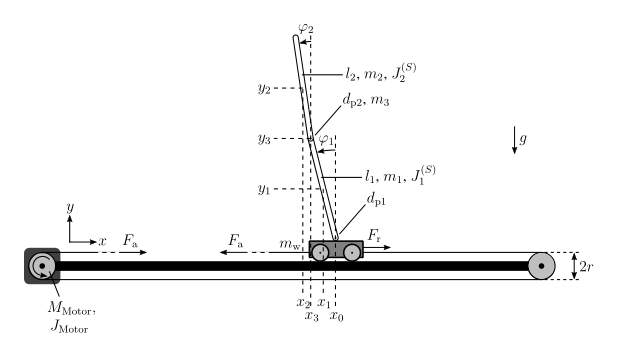
\includegraphics{DPskizze}
		\caption{Aufbau des inversen Doppelpendels EIGENE SKIZZE NOCH ZU ERSTELLEN}
		\label{fig.DPskizze}
	\end{center}
\end{figure}

%\begin{equation}
%sljdsjuhd = luhsdfiuhsf+ spidhfos
%\end{equation}

